%
% Complete documentation on the extended LaTeX markup used for Insight
% documentation is available in ``Documenting Insight'', which is part
% of the standard documentation for Insight.  It may be found online
% at:
%
%     http://www.itk.org/

\documentclass{InsightArticle}

\usepackage[dvips]{graphicx}

%%%%%%%%%%%%%%%%%%%%%%%%%%%%%%%%%%%%%%%%%%%%%%%%%%%%%%%%%%%%%%%%%%
%
%  hyperref should be the last package to be loaded.
%
%%%%%%%%%%%%%%%%%%%%%%%%%%%%%%%%%%%%%%%%%%%%%%%%%%%%%%%%%%%%%%%%%%
\usepackage[dvips,
bookmarks,
bookmarksopen,
backref,
colorlinks,linkcolor={blue},citecolor={blue},urlcolor={blue},
]{hyperref}
\usepackage{subfig}


%  This is a template for Papers to the Insight Journal. 
%  It is comparable to a technical report format.

% The title should be descriptive enough for people to be able to find
% the relevant document. 
\title{Incremental Delaunay Exact Triangulation}

% 
% NOTE: This is the last number of the "handle" URL that 
% The Insight Journal assigns to your paper as part of the
% submission process. Please replace the number "1338" with
% the actual handle number that you get assigned.
%
\newcommand{\IJhandlerIDnumber}{1338}  %TOMODIFY

% Increment the release number whenever significant changes are made.
% The author and/or editor can define 'significant' however they like.
\release{0.01}

% At minimum, give your name and an email address.  You can include a
% snail-mail address if you like.
\author{St\'{e}phane Rigaud$^{1}$ and Alexandre Gouaillard$^{2}$}
\authoraddress{$^{1}$Image \& Pervasive Access Lab, National Centre for Scientific Research (CNRS), Fusionopolis, Singapore\\
               $^{2}$Singapore Immunology Network, Agency for Science, Technology and Research (A*STAR), Biopolis, Singapore}

\begin{document}

%
% Add hyperlink to the web location and license of the paper.
% The argument of this command is the handler identifier given
% by the Insight Journal to this paper.
% 
\IJhandlefooter{\IJhandlerIDnumber}


\ifpdf
\else
   \DeclareGraphicsExtensions{.eps,.jpg,.gif,.tiff,.bmp,.png}
   \DeclareGraphicsRule{.jpg}{eps}{.jpg.bb}{`convert #1 eps:-}
   \DeclareGraphicsRule{.gif}{eps}{.gif.bb}{`convert #1 eps:-}
   \DeclareGraphicsRule{.tiff}{eps}{.tiff.bb}{`convert #1 eps:-}
   \DeclareGraphicsRule{.bmp}{eps}{.bmp.bb}{`convert #1 eps:-}
   \DeclareGraphicsRule{.png}{eps}{.png.bb}{`convert #1 eps:-}
\fi


\maketitle


\ifhtml
\chapter*{Front Matter\label{front}}
\fi


% The abstract should be a paragraph or two long, and describe the
% scope of the document.
\begin{abstract}
\noindent
This document describes the implementation in ITK of the \emph{Incremental Delaunay Triangulation} algorithm. Using the \emph{Straight Walk in Triangulation function} \cite{Rigaud2012}, the \emph{exact discrete geometrical orientation predicate} \cite{Moreau2011},  and the \emph{itk::QuadEdgeMesh} API \cite{Gouaillard2006} of ITK , we propose an efficient, geometrically exact and robust implementation that, from an \emph{itk::PointSet} structure, incrementally construct the Delaunay Triangulation of the \emph{itk::PointSet}.

\end{abstract}

\IJhandlenote{\IJhandlerIDnumber}

\tableofcontents
\vfil
\section{Principle of Incremental Delaunay Triangulation}

Taking a planar set of points $\mathcal{P}$ of $\mathit{n}$ points embedded into a \emph{n}-dimensions space, we construct a triangulation $\mathit{DT(}\mathcal{P}\mathit{)}$, that respect the Delaunay criterion stating that no points of $\mathcal{P}$ should be inside of the circumference circle of any triangle of $\mathit{DT(}\mathcal{P}\mathit{)}$.\\

Several algorithm exist to compute a Delaunay triangulation, the most straightforward way of computing it is the Incremental Delaunay triangulation algorithm. Let $\mathcal{P}$ a point set and $\mathit{DT(} \mathcal{P_{\mathit{t}}} \mathit{)}$ the Delaunay triangulation of $\mathcal{P_{\mathit{t}}}\subset\mathcal{P}$. We construct $\mathit{DT(} \mathcal{P_{\mathit{t+1}}} \mathit{)}$ by adding a point $\mathit{p_{t}}$ randomly taken from $\mathcal{P} \backslash \mathcal{P_{\mathit{t}}}$ into the $\mathit{DT(} \mathcal{P_{\mathit{t}}} \mathit{)}$. Then, the triangle $\mathit{t}$ of $\mathit{DT(} \mathcal{P_{\mathit{t}}} \mathit{)}$ that embed the point $\mathit{p_{t}}$ is located using a Walk in a Triangulation algorithm and subdivide into three new triangle $\mathit{t_{1}}$, $\mathit{t_{2}}$ and $\mathit{t_{3}}$, which share the same vertex $\mathit{p_{t}}$.\\

This triangulation will generate a 2-manifold planar mesh of 1 component and 1 boundary, embedded into a \emph{n}-dimensions space, that will respect the Delaunay criterion.

\section{Implementation}

The algorithm is implemented as a class filter that take an \emph{itk::PointSet} as input and generate an \emph{itk::QuadEdgeMesh} as output. In order to respect the ITK template implementation, we added a new inheritance branch for our filter (Fig. \ref{fig:inheritance}). Where the \emph{itk::PointSetToQuadEdgeMeshFilter} is mainly inspired from the existing \emph{itk::MeshToMeshFilter} but where only the points information of the input are copied to the output.

\begin{figure}
\center
\includegraphics[width=\textwidth]{inheritance}
\itkcaption{Inheritance diagram.}
\label{fig:inheritance}
\end{figure}

\subsection{Initialisation}

The Incremental algorithm is a step case algorithm which need an initialisation step. We initialise $\mathit{DT(}\mathcal{P}_{0}\mathit{)}$ by creating a four points mesh which enclose all the points of $\mathcal{P}$. Those four points $\Omega_{0}$, $\Omega_{1}$, $\Omega_{2}$ and $\Omega_{3}$ are at the extremity of the coordinates space of $\mathcal{P}$ (Fig. \ref{fig:algo1}). This is to make sure that their edges will always respect the criterion and will not influence the triangulation. Once the algorithm has converge, the points are removed with all edges related to them (Fig. \ref{fig:algo6}).

\subsection{The loop}

\subsubsection{Adding a point}

At each step of the algorithm, we add a new point $\mathit{p_{t}}$ to the triangulation (Fig. \ref{fig:algo3}). First we locate the triangle $\mathit{T}(\mathit{p_{i}},\mathit{p_{j}},\mathit{p_{k})}$ of the current triangulation $\mathit{DT(}\mathcal{P}_{\mathit{t}}\mathit{)}$ the point $\mathit{p_{t}}$ is going to affect. This is done using the \emph{itk::WalkInTriangulationFunction} \cite{Rigaud2012}. The triangle $\mathit{T}$ is remove and replace by the three triangles $\mathit{T}_{1}(\mathit{p_{i}},\mathit{p_{j}},\mathit{p_{t})}$, $\mathit{T}_{2}(\mathit{p_{j}},\mathit{p_{k}},\mathit{p_{t})}$ and $\mathit{T}_{3}(\mathit{p_{k}},\mathit{p_{i}},\mathit{p_{t})}$ (Fig. \ref{fig:algo4}).

\subsubsection{Criterion Check}

The Delaunay criterion is then check for the newly created triangle $\mathit{T}_{1}$, $\mathit{T}_{2}$ and $\mathit{T}_{3}$ (Fig. \ref{fig:algo5}). It use the \emph{itk::PointInCircleGeometricalPredicateFunctor} \cite{Moreau2011} and verify, for the given triangle and point, the emptiness of the circumference circle for the adjacent face and opposite to the given point. If the face is not respectful of the criterion, we \emph{flip} the diagonal edge of the quadrilater formed by the triangle and its adjacent triangle using the \emph{itk::QuadEdgeMeshFlipEdgeEulerOperator}. Because the \emph{flip} can affect the validity of other local edge, the verification is recursively called on the two new triangles created from the edge flipping.

\begin{figure}
\center
\subfloat[]{\label{fig:algo1}\includegraphics[width=0.25\textwidth]{1a}} 
\subfloat[]{\label{fig:algo2}\includegraphics[width=0.25\textwidth]{2a}} 
\subfloat[]{\label{fig:algo3}\includegraphics[width=0.25\textwidth]{3a}} \hspace{5pt}
\subfloat[]{\label{fig:algo4}\includegraphics[width=0.25\textwidth]{4a}}
\subfloat[]{\label{fig:algo5}\includegraphics[width=0.25\textwidth]{5a}}
\subfloat[]{\label{fig:algo6}\includegraphics[width=0.25\textwidth]{6a}}
\itkcaption{Incremental algorithm iteration. (a) Initialisation step. (b) $\mathit{DT(}\mathcal{P}_{\mathit{t}}\mathit{)}$. (c) Add a point $\mathit{p}_{\mathit{t}}$ to $\mathit{DT(}\mathcal{P}_{\mathit{t}}\mathit{)}$. (d) Create three new triangles $\mathit{T}_{1}$, $\mathit{T}_{2}$ and $\mathit{T}_{3}$. (d) Flip illegal edge in order to obtain $\mathit{DT(}\mathcal{P}_{\mathit{t+1}}\mathit{)}$. (e) Remove temporary points from the initialisation step.}
\label{fig:Algo}
\end{figure}

\section{Usage}

An example \texttt{DelaunayIncremental.cxx} is provided with the sources and is used for the tests. The filter is templated on 2 dimensions \textit{itk::PointSet} and \textit{itk::QuadEdgeMesh}, if a higher dimensions mesh or set of points is given, only the two first dimension will be used in the process. Some points configuration generator are provided with the sources for the testing.

\begin{verbatim}
typedef itk::PointSet< PixelType, Dimension > TPointSet;
typedef itk::QuadEdgeMesh< PixelType, Dimension > TQuadEdgeMesh;
typedef itk::PointSetToQuadEdgeMeshFilter< TPointSet, TQuadEdgeMesh > MyFilter;

TPointSet::Pointer pointset = TPointSet::New();
TQuadEdgeMesh::Pointer triangulation = TQuadEdgeMesh::New();

MyFilter::Pointer myFilter = MyFilter::New();
myFilter->SetInput( pointset );
triangulation = myFilter->GetOutput();
myFilter->Update();
\end{verbatim}

The validation of the filter output is made using the \emph{itk::DelaunayConformingQuadEdgeMeshFilter}, by quantifying how many edge flip was necessary to make the filter output mesh Delaunay conform. The number of edge flip done by the \emph{itk::DelaunayConformingQuadEdgeMeshFilter} is expected to be equal to zero.

\begin{figure}
\center
\subfloat[]{\label{fig:res1}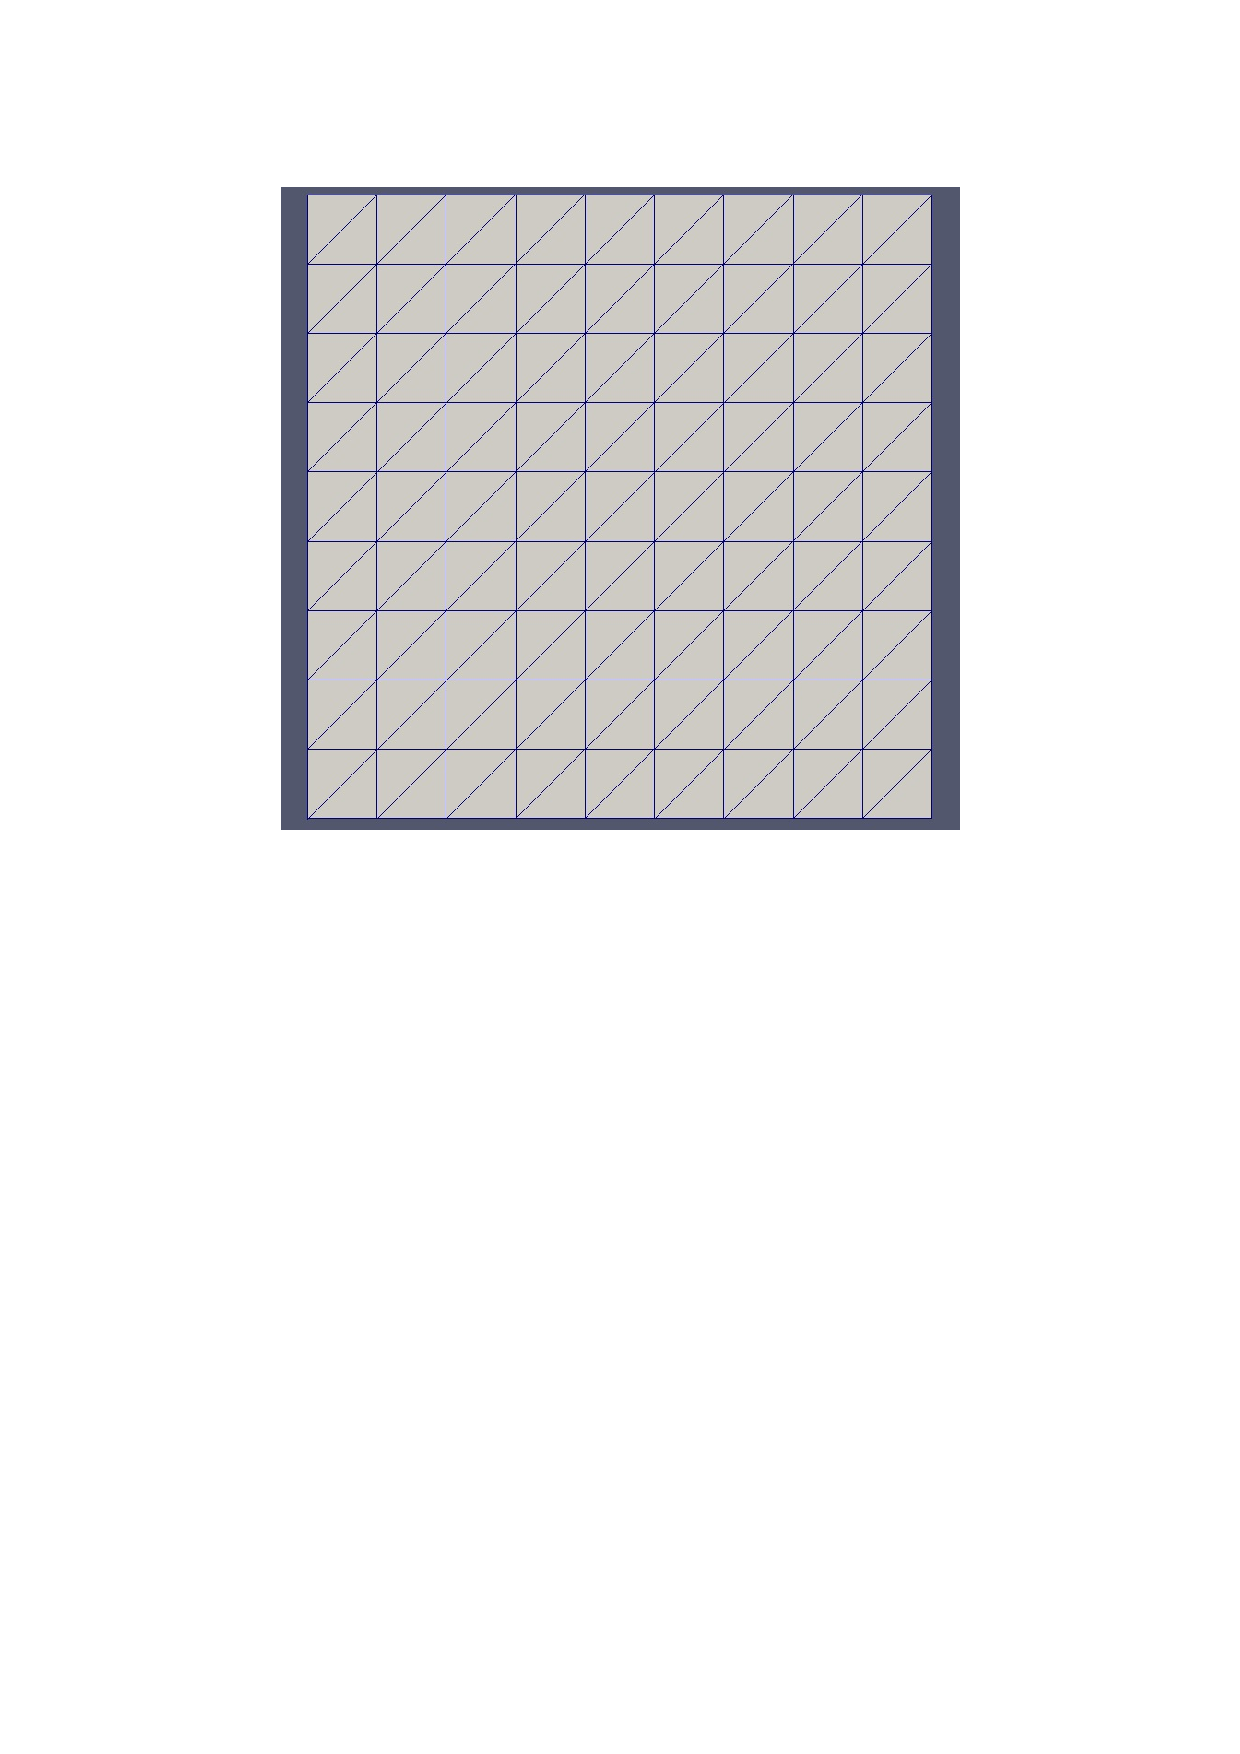
\includegraphics[width=0.45\textwidth]{1r}}  \hspace{5pt}
\subfloat[]{\label{fig:res2}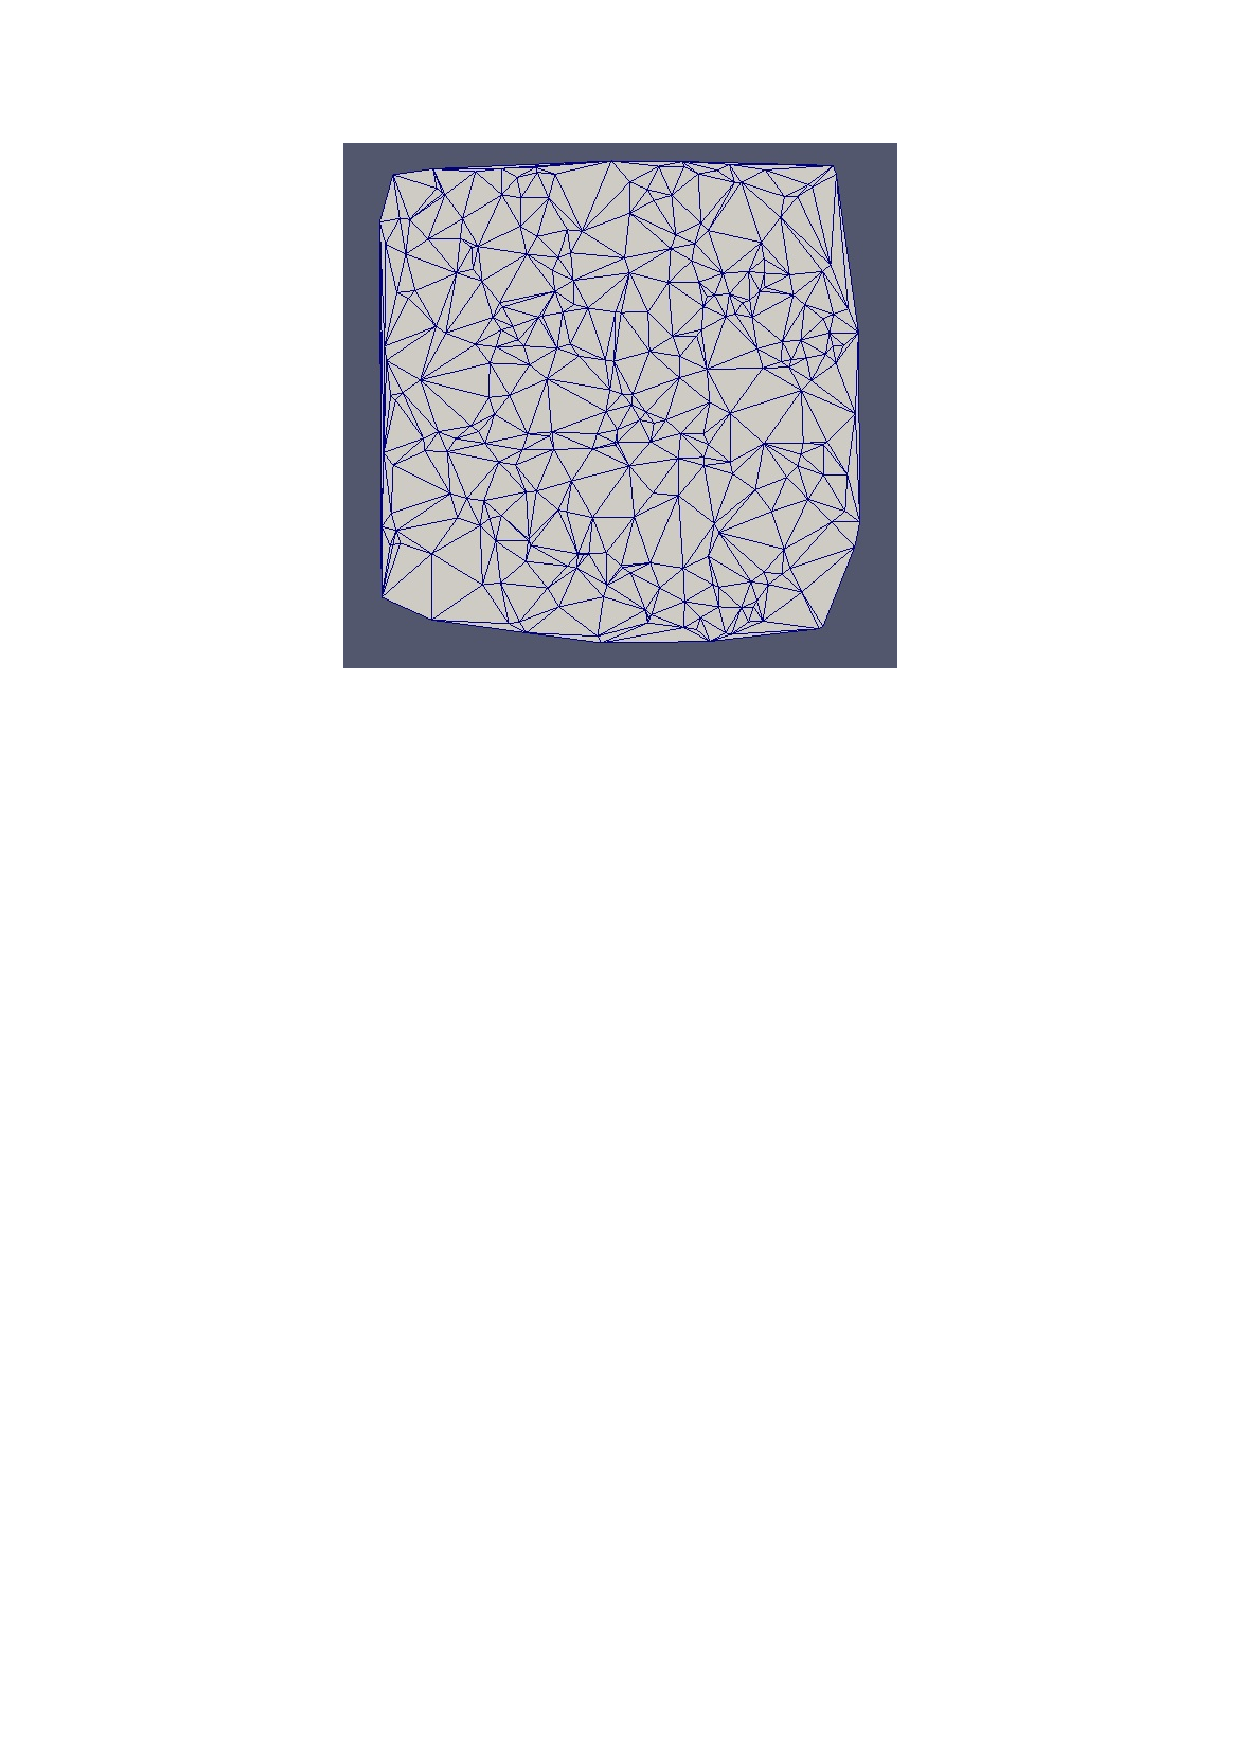
\includegraphics[width=0.45\textwidth]{2r}} 
\itkcaption{Paraview displays of random results.}
\label{fig:res}
\end{figure}

%%%%%%%%%%%%%%%%%%%%%%%%%%%%%%%%%%%%%%%%%
%
%  Insert the bibliography using BibTeX
%
%%%%%%%%%%%%%%%%%%%%%%%%%%%%%%%%%%%%%%%%%

\bibliographystyle{plain}
\bibliography{InsightJournal}

\end{document}

